\section{Applications}
\begin{frame}
    \frame{\frametitle{Generative Adversarial Networks - Some Cool Stuff and Applications}}
	% \myheading{Module 23.4: Generative Adversarial Networks - Some Cool Stuff and Applications}
\end{frame}

\begin{frame}
	\begin{figure}[h!]
		%\vspace*{-1mm}
		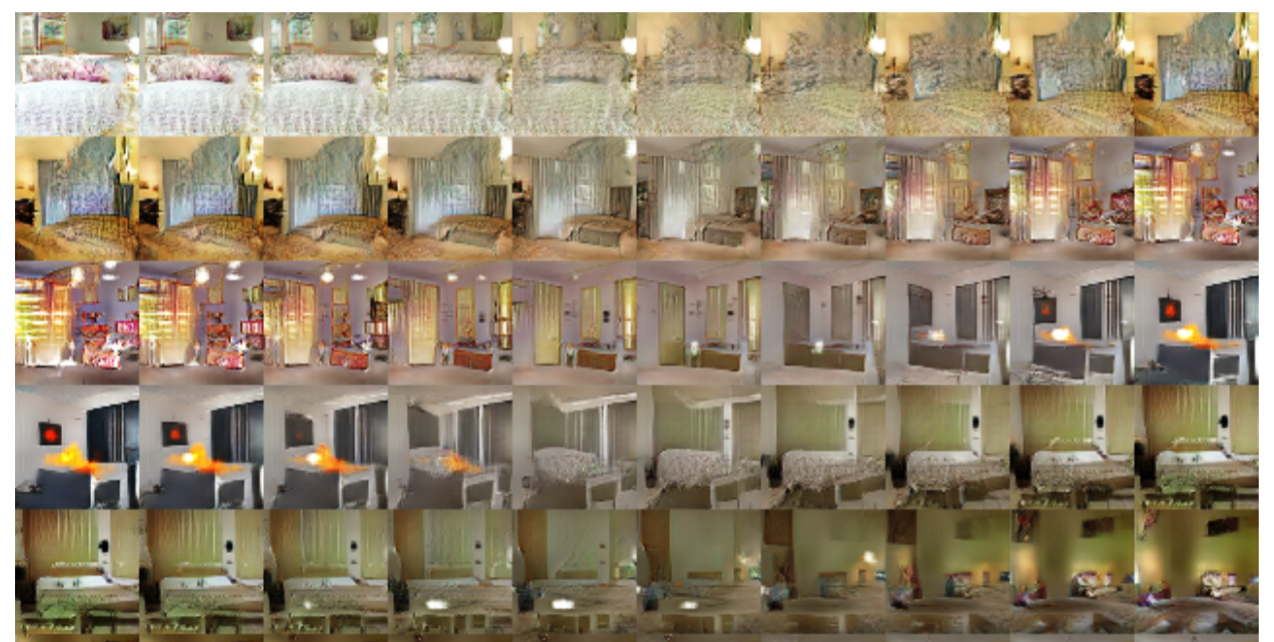
\includegraphics[scale=0.40]{images/Interpolation.png}
		%\vspace*{-4mm}
	\end{figure}
	\begin{itemize}
		\item<1-> In each row the first image was generated by the network by taking a vector $z_1$ as the input and the last images was generated by a vector $z_2$ as the input
		\item<2-> All intermediate images were generated by feeding $z$'s which were obtained by interpolating $z_1$ and $z_2$ ($z = \lambda z_1 + (1-\lambda)z_2$)
		\item<3-> As we transition from $z_1$ to $z_2$ in the input space there is a corresponding smooth transition in the image space also
	\end{itemize}
\end{frame}

\begin{frame}
	\begin{figure}[h!]
		%\vspace*{-1mm}
		\includegraphics<1-4>[scale=0.40]{images/Smiling.png}
		\includegraphics<5->[scale=0.40]{images/Glasses.png}%\vspace*{-4mm}
        \caption{Vector arithmetic for visual concepts (part of figure 7 from the DCGAN paper)}
	\end{figure}
	\begin{itemize}
		\item<1-> The first 3 images in the first column were generated by feeding some $z_{11}, z_{12}, z_{13}$ respectively as the input to the generator
		\item<2-> The fourth image was generated by taking an average of $z_1 = z_{11}, z_{12}, z_{13}$ and feeding it to the generator 
		\item<3-> Similarly we obtain the average vectors $z_2$ and $z_3$ for the 2nd and 3rd columns
		\item<4-> If we do a simple vector arithmetic on these averaged vectors then we see the corresponding effect in the generated images
	\end{itemize}
\end{frame}

\begin{frame}
	\begin{figure}[h!]
		%\vspace*{-1mm}
		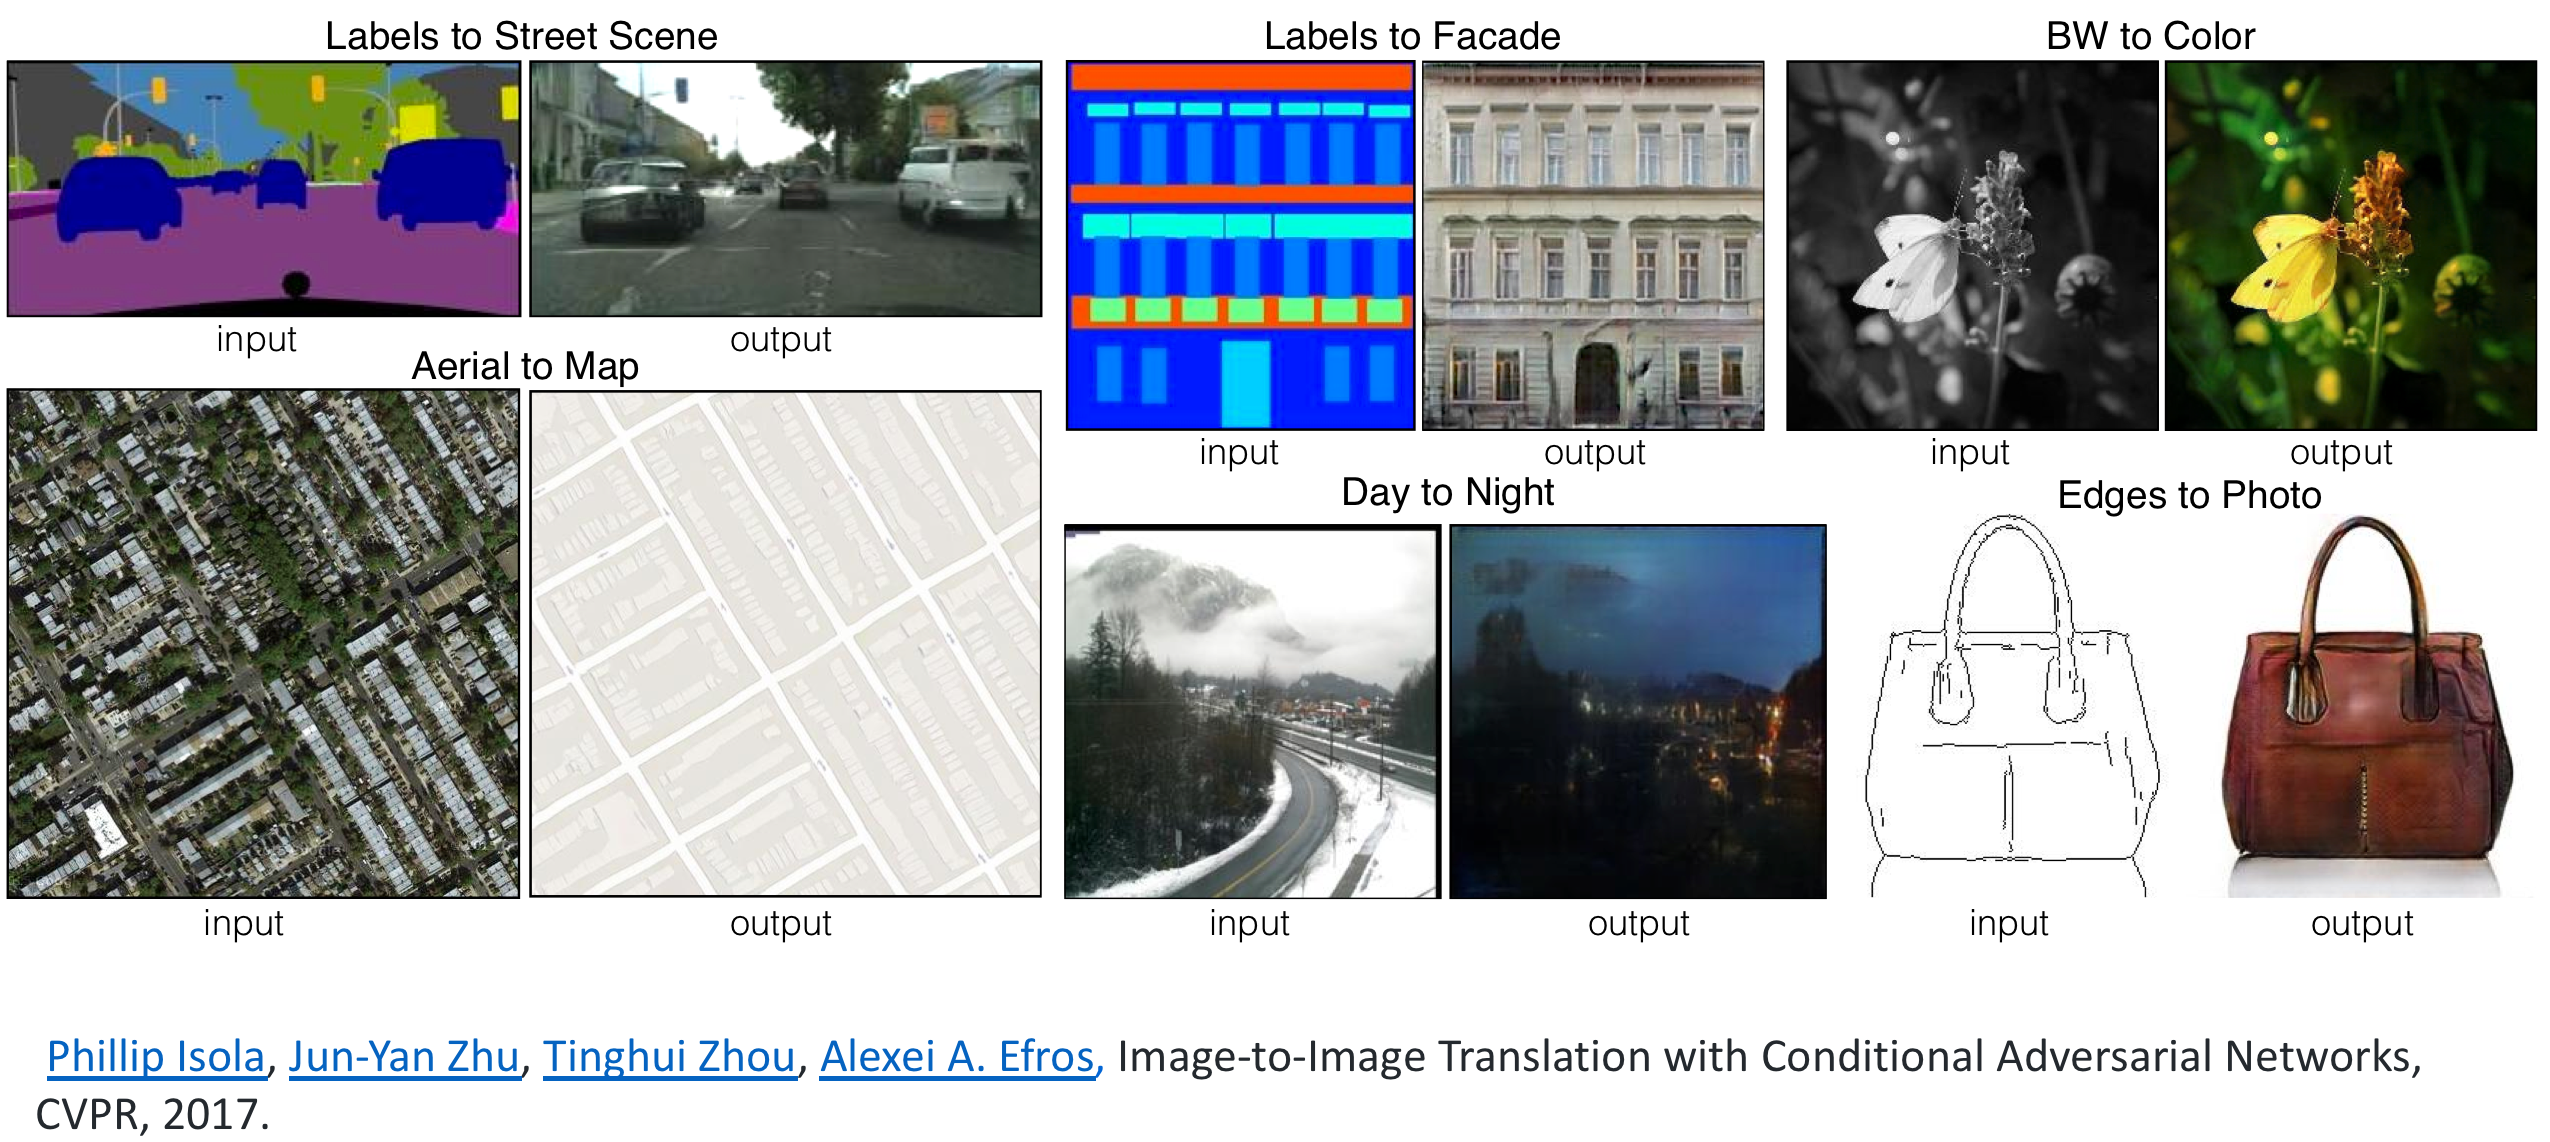
\includegraphics[scale=0.20]{images/GAN_Applications.png}
		%\vspace*{-4mm}
	\end{figure}
\end{frame}

\if 0
\begin{frame}
	\textbf{Various Applications of GAN :}
	\vspace*{2mm}
	\begin{columns}
		\column{0.5\textwidth}
		\hspace*{6mm}\textcolor{red}{\textit{Better training and generation}}
			\begin{overlayarea}{\textwidth}{\textheight}
				\begin{center}
					\begin{figure}[h!]
						\vspace*{-1mm}
						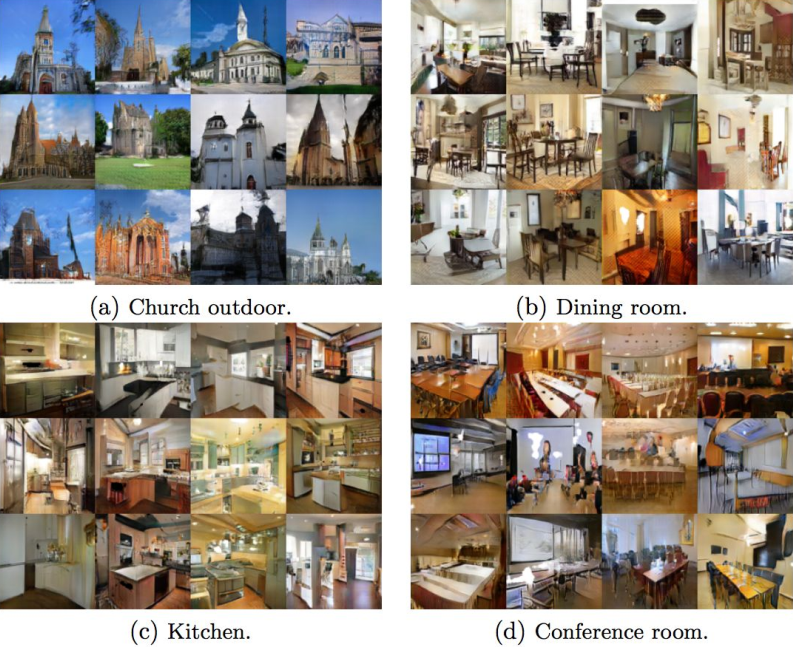
\includegraphics[scale=0.15]{images/lsgan.png}
						\vspace*{-4mm}
						\caption{LSGAN. Mao et al. 2017}
					\end{figure}
					\begin{figure}[h!]
						\vspace*{-4mm}
						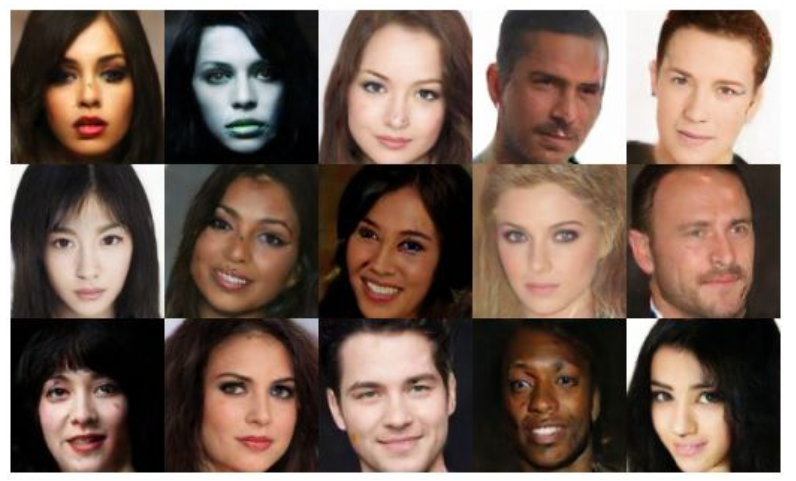
\includegraphics[scale=0.15]{images/began.png}
						\vspace*{-4mm}
						\caption{BEGAN. Bertholet et al. 2017}
					\end{figure}
				\end{center}
			\end{overlayarea}
		\column{0.5\textwidth}
		
			\begin{overlayarea}{\textwidth}{\textheight}
			\only<2->{
			\hspace*{6mm}\textcolor{red}{\textit{Source $\rightarrow$ Target domain transfer}}
				\begin{center}
					\begin{figure}[h!]
						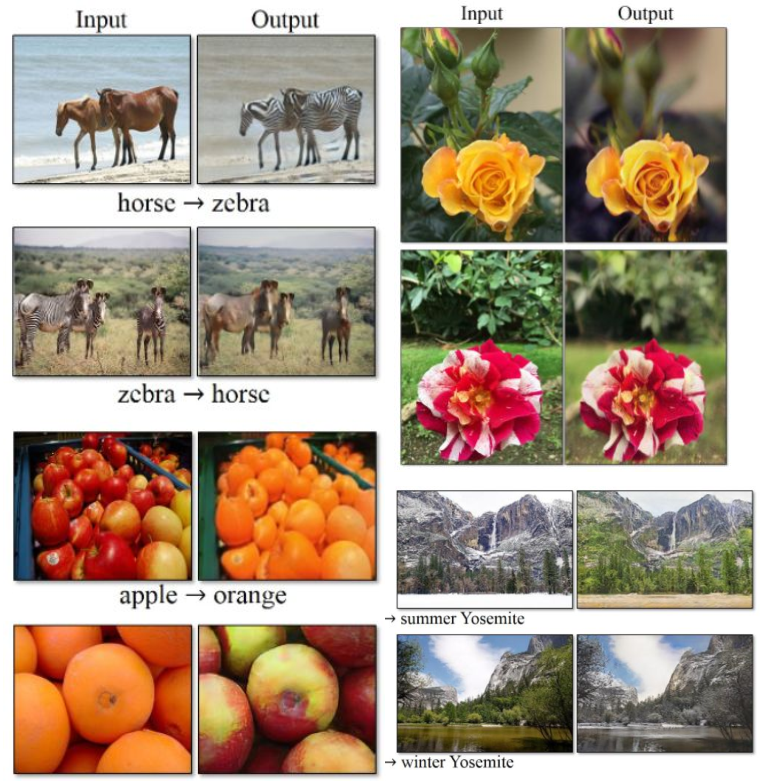
\includegraphics[scale=0.15]{images/cyclegan.png}
						\vspace*{-4mm}
						\caption{CycleGAN. Zhu et al. 2017}
					\end{figure}
				\end{center}}
			\end{overlayarea}
	\end{columns}
\end{frame}

\begin{frame}
\textbf{Various Applications of GAN :}
	\vspace*{2mm}
	\begin{columns}

		\column{0.5\textwidth}
			\begin{overlayarea}{\textwidth}{\textheight}
			\hspace*{6mm}
			\textcolor{red}{\textit{Text $\rightarrow$ Image Synthesis}}
				\begin{center}
				\begin{figure}[h!]

					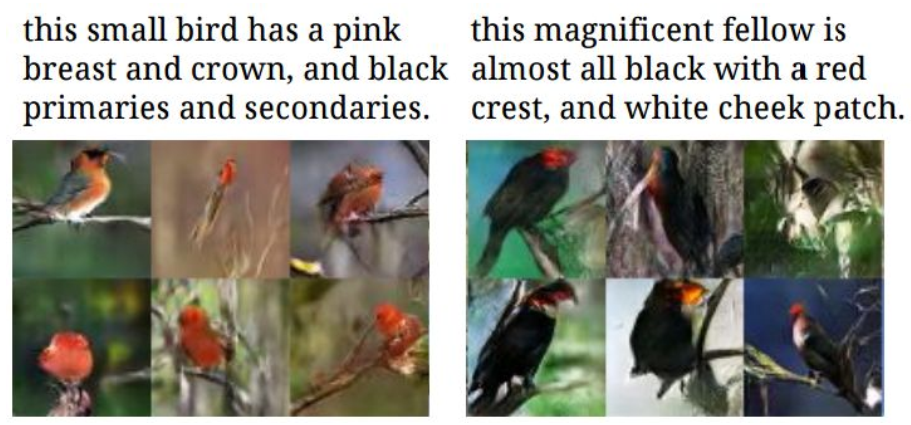
\includegraphics[scale=0.15]{images/image-synthesis.png}
					\vspace*{-4mm}
					\caption{Reed et al. 2017}
				\end{figure}
				\end{center}
			\end{overlayarea}
			
		\column{0.5\textwidth}
			\begin{overlayarea}{\textwidth}{\textheight}
			\only<2->{
			\hspace*{6mm}			
			\textcolor{red}{\textit{Many GAN applications}}
				\begin{center}
				\begin{figure}[h!]
					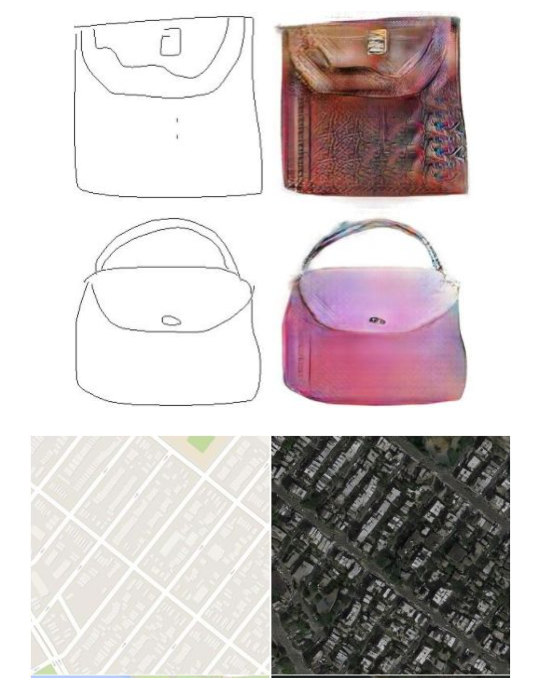
\includegraphics[scale=0.15]{images/pix2pix.png}
					\vspace*{-4mm}
					\caption{Pix2pix. Isola 2017.}
				\end{figure}
				\end{center}}
			\end{overlayarea}
						
	\end{columns}
\end{frame}

\begin{frame}
	\begin{overlayarea}{\textwidth}{\textheight}
	\begin{table}[]
	\def\arraystretch{1.5}%
\resizebox{0.8\textwidth}{!}{%
\begin{tabular}{c|cccc}
             & RBMs                  & VAEs                  & AR models     & GANs        \\
%\hline
%\hline
\toprule
Abstraction  & Yes                   & Yes                   & No            & No          \\
\onslide<2->{Generation}   & \onslide<2->{Yes                   & Yes                   & Yes           & Yes}         \\
\onslide<3->{Compute P(X)} & \onslide<3->{Intractable           & Intractable           & Tractable     & No }         \\
\onslide<4->{Sampling     }& \onslide<4->{MCMC                  & Fast                  & Slow          & Fast }       \\
\onslide<5->{Type of GM  } & \onslide<5->{Undirected            & Directed              & Directed      & Directed}    \\
\onslide<6->{Loss       }  & \onslide<6->{KL-divergence         & KL-divergence         & KL-divergence & JSD }        \\
\onslide<7->{Assumptions}  & \onslide<7->{X independent given z & X independent given z & None          & N.A. }       \\
\onslide<8->{Samples}      & \onslide<8->{Bad                   & Ok                    & Good          & Good (best)} \\
\bottomrule
\end{tabular}}
\caption{Comparison of Generative Models}
\label{my-label}
\end{table}
\only<9->{
\small
\textit{
Recent works look at combining these methods: e.g. Adversarial Autoencoders (Makhzani 2015), PixelVAE (Gulrajani 2016) and PixelGAN Autoencoders (Makhzani 2017)}}

	\end{overlayarea}
\end{frame}
\fi

